다음 그림과 같은 $\triangle\mathrm{ABC}$에서 $\angle\mathrm{A}$, $\angle\mathrm{C}$의 외각의 이등분선의 교점을 $\mathrm{O}$, 점 $\mathrm{O}$에서 $\overline{\mathrm{BA}}$의 연장선과 $\overline{\mathrm{BC}}$의 연장선에 내린 수선의 발을 $\mathrm{D}$, $\mathrm{E}$라고 하자. $\overline{\mathrm{AB}} = 7\,\mathrm{cm}$, $\overline{\mathrm{BC}} = 10\,\mathrm{cm}$, $\overline{\mathrm{AC}} = 5\,\mathrm{cm}$일 때, $\overline{\mathrm{CE}}$의 길이는 몇 $\mathrm{cm}$인지 구하여라.

\begin{figure}[h]
\centering
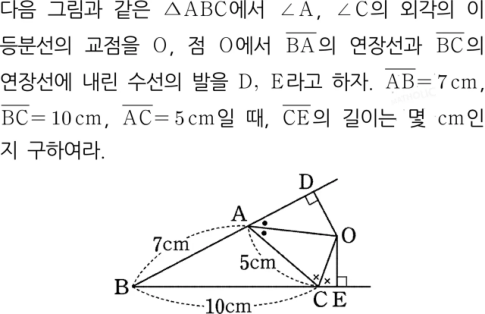
\includegraphics[width=0.4\textwidth]{plain0_problem_10_figure.png}
\end{figure}
